 \section*{Topics}  \begin{DoxyItemize}
\item \hyperlink{overview}{Overview of Base\+Ten} \item \hyperlink{baseten_assistant}{Base\+Ten Assistant} \item \hyperlink{getting_started}{Getting started} \item \hyperlink{accessing_values}{Accessing object values} \item \hyperlink{sql_views}{S\+Q\+L views} \item \hyperlink{database_types}{Handled Postgre\+S\+Q\+L types} \item \hyperlink{relationships}{Relationships} \item \hyperlink{predicates}{Predicates} \item \hyperlink{tracking_changes}{Tracking database changes} \item \hyperlink{using_appkit_classes}{Using Base\+Ten\+App\+Kit} \item \hyperlink{autocommit_manual_commit}{Commit modes and locking} \item \hyperlink{thread_safety}{Thread safety} \item \hyperlink{multiple_contexts}{Using multiple database contexts} \item \hyperlink{linking_to_baseten}{Linking to Base\+Ten and Base\+Ten\+App\+Kit} \item \hyperlink{building_baseten}{Building Base\+Ten} \end{DoxyItemize}
\hypertarget{overview}{}\section{Overview of Base\+Ten}\label{overview}
Base\+Ten aims to provide a Core Data -\/like A\+P\+I for handling a database. A database connection is managed by an instance of B\+X\+Database\+Context, which also fetches rows from the database. Rows are represented by instances of \hyperlink{interface_b_x_database_object}{B\+X\+Database\+Object}. Objects are identified by \hyperlink{interface_b_x_database_object_i_d}{B\+X\+Database\+Object\+I\+Ds}, that are created using tables' primary keys. Foreign keys are interpreted as relationships between objects.

Like some other object-\/relational mappers, Base\+Ten fetches the data model from the database. There are classes available for database introspection\+: \hyperlink{interface_b_x_entity_description}{B\+X\+Entity\+Description}, \hyperlink{interface_b_x_attribute_description}{B\+X\+Attribute\+Description}, \hyperlink{interface_b_x_relationship_description}{B\+X\+Relationship\+Description} and its subclasses.

Database objects are retrieved using an instance of B\+X\+Database\+Context. The rows are specified using instances of \hyperlink{interface_b_x_entity_description}{B\+X\+Entity\+Description} and N\+S\+Predicate. This pattern should match most use cases. It is also possible to fetch rows as N\+S\+Dictionaries by specifying an S\+Q\+L query.

Unlike the typical use case of Core Data, multiple users might be connected to the database being accessed using Base\+Ten. Thus, data manipulated with database objects could change at any time. Base\+Ten copes with this situation by updating objects' contents as soon as other database clients commit their changes. The other clients needn't use Base\+Ten.

Instead of constantly polling the database for changes, Base\+Ten listens for Postgre\+S\+Q\+L notifications. It then queries the database about the notification type and faults the relevant objects. For this to work, certain tables, views and functions need to be created in the database. The easiest way to do this is to connect to the database with Base\+Ten Assistant. Using it, relations may be enabled for use with the framework. Everything will be installed or will reference to a database schema called baseten, so removal, if needed, will be an easy process. Base\+Ten can connect to databases without the schema, but in this case functionality will be limited.

Since Base\+Ten relies on database introspection, S\+Q\+L may be used to define the database schema. Another option is to create a data model using Xcode's data modeler and import it using Base\+Ten Assistant.


\begin{DoxyImage}
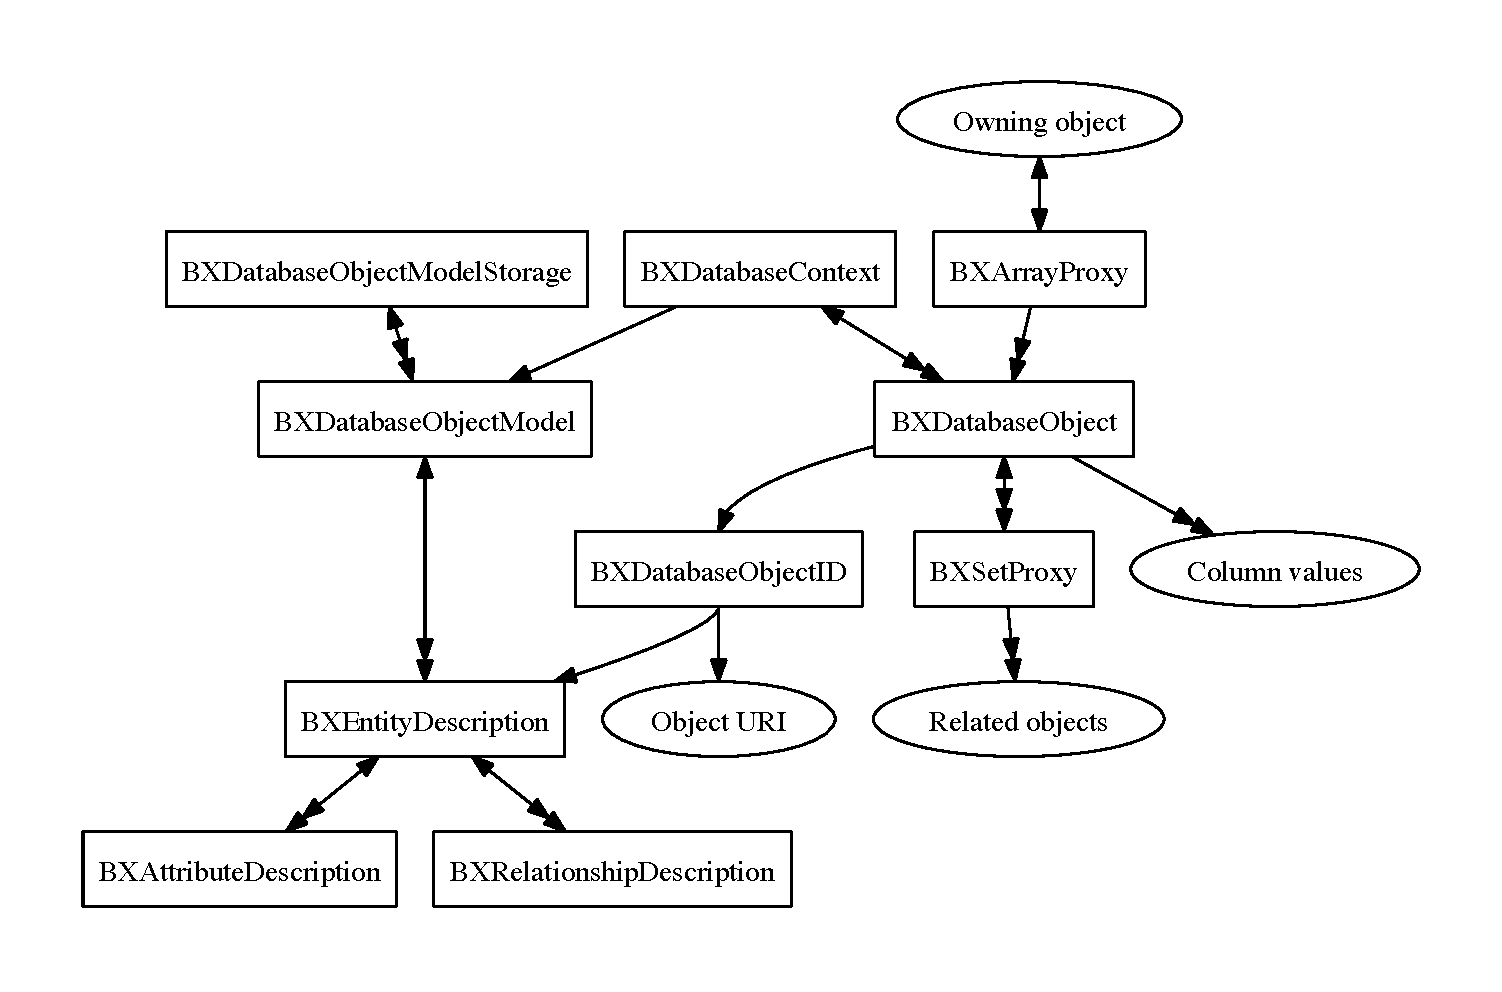
\includegraphics[width=\textwidth]{object-relationships}
\caption{Relationships between Base\+Ten's objects}
\end{DoxyImage}
 
\begin{DoxyImage}
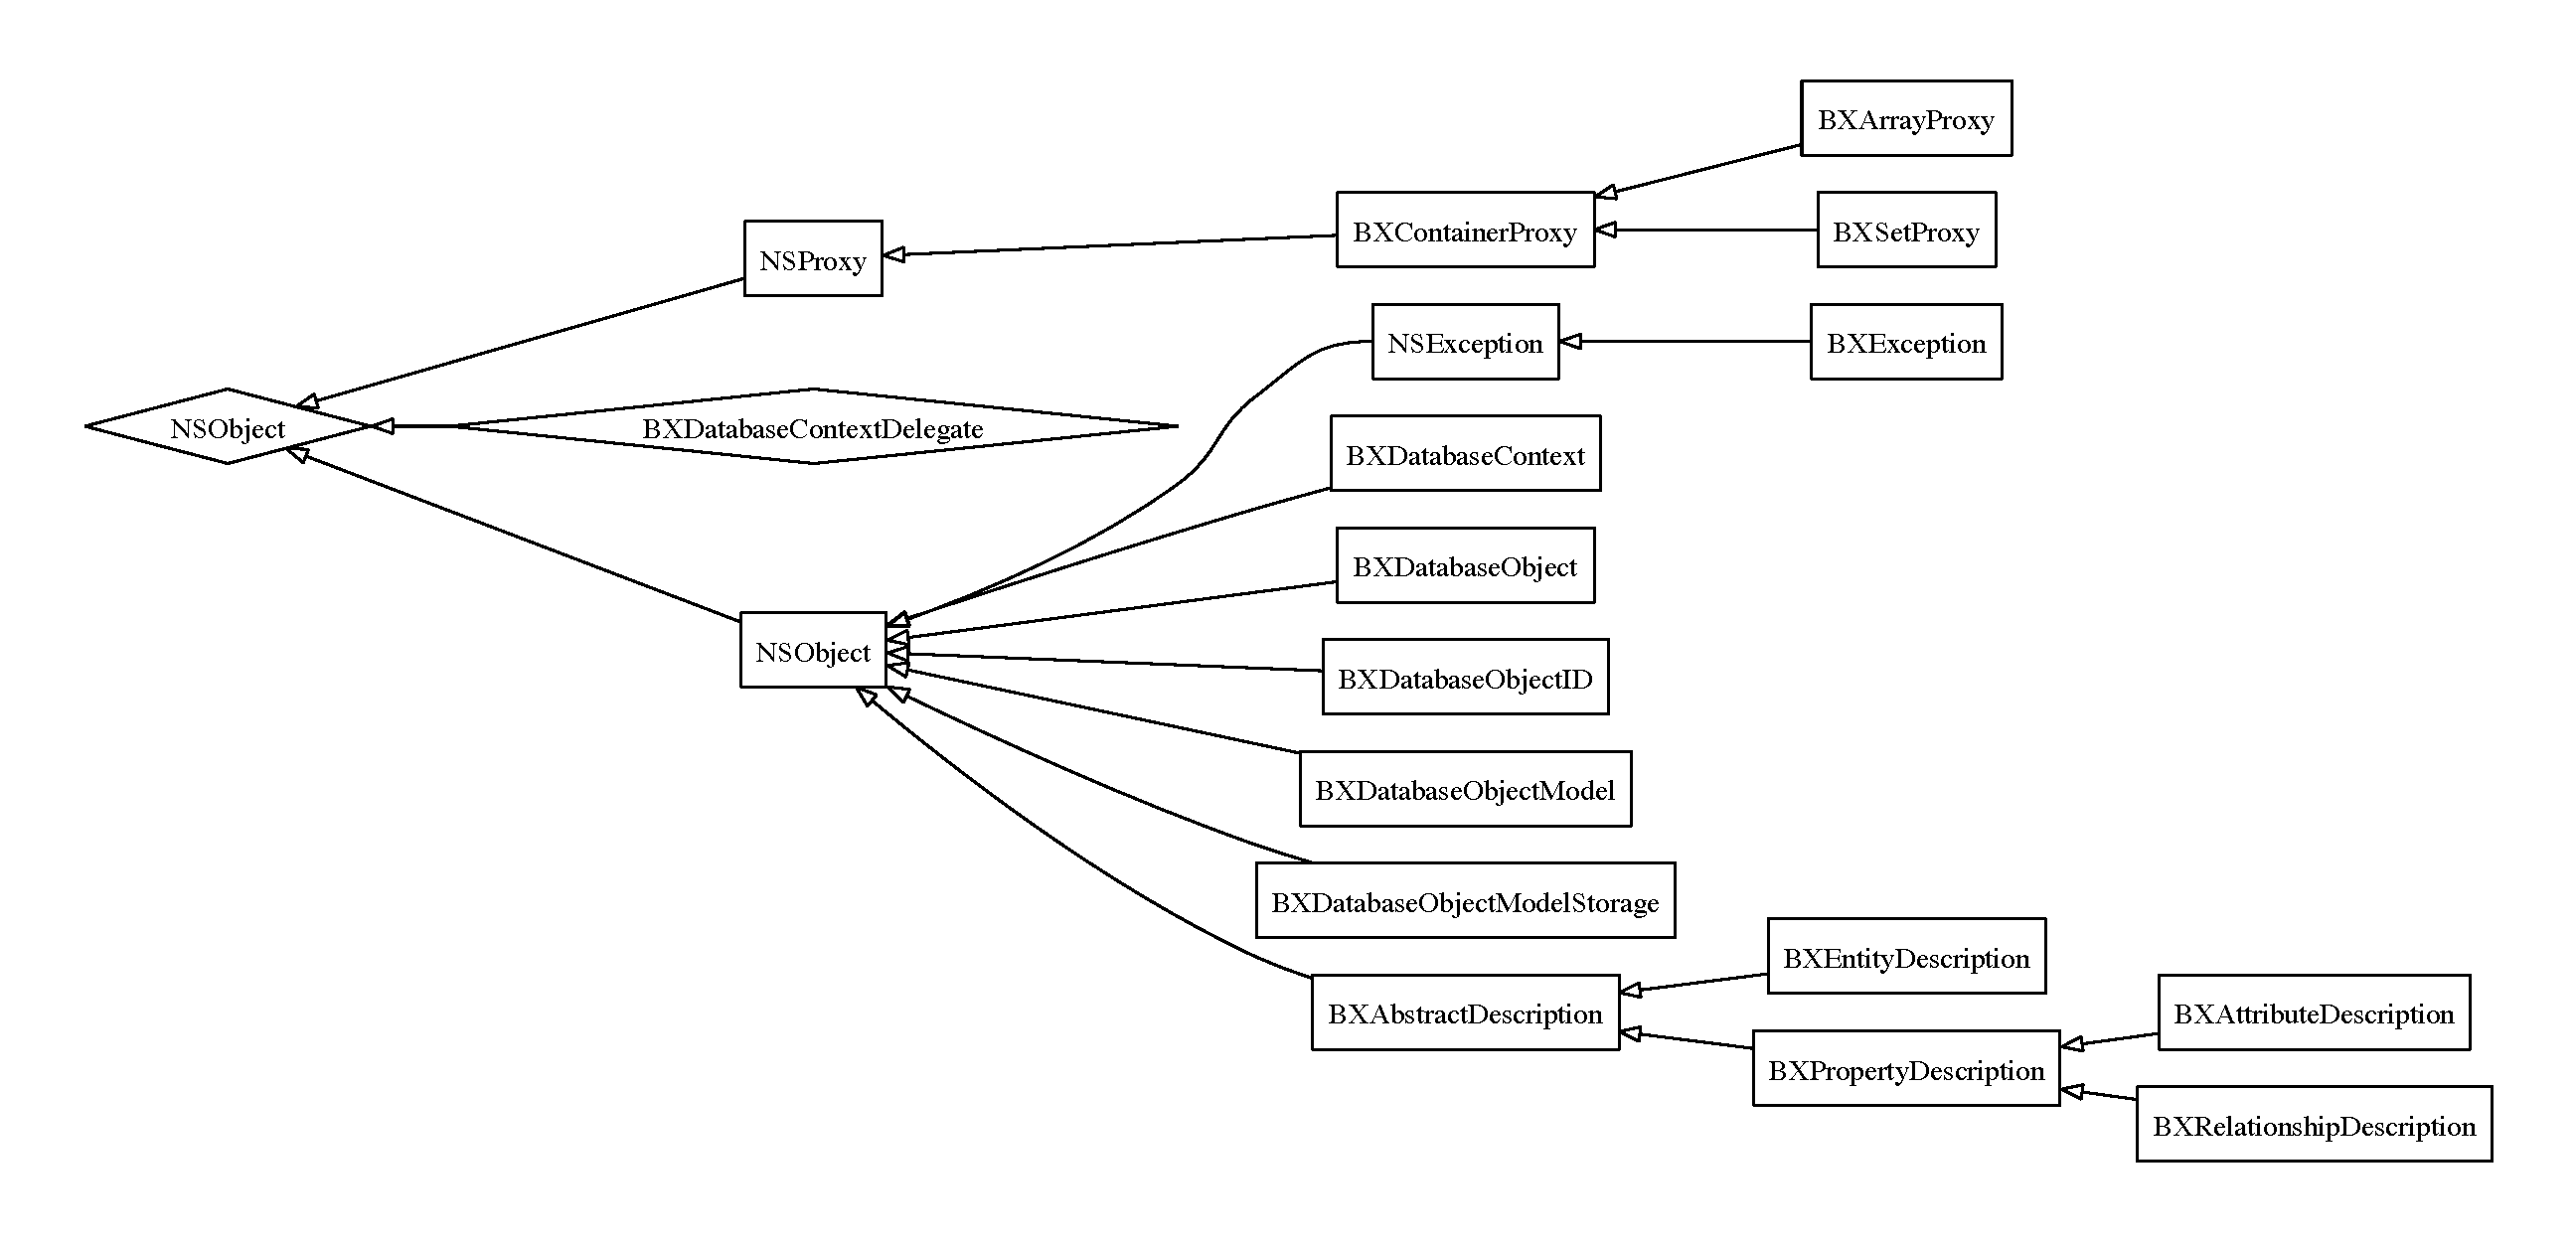
\includegraphics[width=\textwidth]{class-hierarchy}
\caption{Base\+Ten class hierarchy}
\end{DoxyImage}
 \hypertarget{baseten_assistant}{}\section{Base\+Ten Assistant}\label{baseten_assistant}
Base\+Ten Assistant is a simple database management application distributed with Base\+Ten framework. It has its own help that is available from within the application. In short, it has the following features\+: \begin{DoxyItemize}
\item It can be used to enable or disable tables and views for use with Base\+Ten. \item It can refresh the tables that Base\+Ten uses to determine relationships between entities. \item It can list entities' attributes and relationships as they are available when using the framework. \item It can create a database schema from an Xcode data model. \item It can create a chart of the database schema that can be displayed using Graphviz or Omni\+Graffle. \end{DoxyItemize}
\hypertarget{getting_started}{}\section{Getting started}\label{getting_started}
Typically accessing a database consists roughly of the following steps\+: 
\begin{DoxyItemize}
\item \hyperlink{getting_started_creating_a_database_context}{Creating an instance of B\+X\+Database\+Context} 
\item \hyperlink{getting_started_connecting_to_a_database}{Connecting to a database} 
\item \hyperlink{getting_started_getting_an_entity_and_a_predicate}{Getting an entity description from the context and possibly creating an N\+S\+Predicate for reducing the number of fetched objects} 
\item \hyperlink{getting_started_performing_a_fetch}{Performing a fetch using the entity and the predicate} 
\item \hyperlink{getting_started_handling_the_results}{Handling the results} 
\item \hyperlink{getting_started_creating_objects}{Creating new objects} 
\end{DoxyItemize}Here is a small walkthrough with sample code. More examples are available in the Base\+Ten Subversion repository and at \href{http://basetenframework.org}{\tt http\+://basetenframework.\+org}.

 
  \lstset{language=[Objective]C, backgroundcolor=\color[rgb]{0.84,0.87,0.90}, rulecolor=\color[gray]{0.53}, frame=single, framesep=0pt, framextopmargin=2pt, framexbottommargin=2pt, fontadjust, columns=fullflexible, captionpos=b}
  \begin{lstlisting}[caption=A simple command line tool that uses BaseTen]
  #import <Foundation/Foundation.h>
  #import <BaseTen/BaseTen.h>
 
  int main (int argc, char** argv)
  {
      NSURL* databaseURI = [NSURL URLWithString: @"pgsql://username@localhost/database"];
      BXDatabaseContext* ctx = [[BXDatabaseContext alloc] initWithDatabaseURI: databaseURI];
  
      [ctx connectSync: NULL];
      BXEntityDescription* entity = [[ctx databaseObjectModel] entityForTable: @"table"];
      NSArray* result = [ctx executeFetchForEntity: entity withPredicate: nil error: NULL];
 
      for (BXDatabaseObject* object in result)
      {
          NSLog (@"Object ID: %@ column: %@", 
                 [[object objectID] URIRepresentation], [object valueForKey: @"column"]);
      }
 
      NSDictionary* values = [NSDictionary dictionaryWithObject: @"newValue" forKey: @"column"];
      BXDatabaseObject* newObject = [ctx createObjectForEntity: entity 
                                      withFieldValues: values error: NULL];
      NSLog (@"new object: %@", newObject);
 
      return 0;
  }
  \end{lstlisting} 
   \hypertarget{getting_started_creating_a_database_context}{}\subsection{Creating a database context}\label{getting_started_creating_a_database_context}
The designated initializer of B\+X\+Database\+Context is -\/init\+With\+Database\+U\+R\+I\+:. -\/init is also available but the context does require an U\+R\+I before connecting.

B\+X\+Database\+Context requires the U\+R\+I to be formatted as follows\+:~\newline
 {\ttfamily pgsql\+://username\+:password@host/database\+\_\+name}. Currently, as Postgre\+S\+Q\+L is the only supported database, only {\ttfamily pgsql\+://} U\+R\+Is are allowed. In command line tools, all parameters are required except for the password, the need for which depends on the database configuration.

Various methods in B\+X\+Database\+Context take a double pointer to an N\+S\+Error object as a parameter. if the called method fails, the N\+S\+Error will be set on return. If the parameter is N\+U\+L\+L, the default error handler raises a \hyperlink{interface_b_x_exception}{B\+X\+Exception}. B\+X\+Database\+Context's delegate may change this behaviour.\hypertarget{getting_started_connecting_to_a_database}{}\subsection{Connecting to a database}\label{getting_started_connecting_to_a_database}
 
  \begin{lstlisting}
  [ctx connectSync: NULL];
  \end{lstlisting}
   

Connection to the database may be made synchronously using the method -\/connect\+Sync. Applications that use an N\+S\+Run\+Loop also have the option to use -\/connect\+Async. The method returns immediately. When the connection attempt has finished, the context's delegate will be called and notifications will be posted to the context's notification center (accessed with -\/notification\+Center).

In App\+Kit applications, the easiest way to connect to the database is to use the I\+B\+Action -\/connect\+:. In addition to attempting the connection asynchronously, it also presents a number of panels to the user, if some required information is missing from the U\+R\+I. The panels allow the user to specify their username, password and the database host making U\+R\+Is like {\ttfamily pgsql\+:///{\itshape database\+\_\+name}} allowed. Additionally a {\itshape k\+B\+X\+Connection\+Setup\+Alert\+Did\+End\+Notification} will be posted when the user dismisses an alert panel, which is presented on failure.

Since {\itshape N\+U\+L\+L} is passed in place of an N\+S\+Error double pointer, a \hyperlink{interface_b_x_exception}{B\+X\+Exception} will be thrown on error. See B\+X\+Database\+Context's documentation for details on error handling.\hypertarget{getting_started_getting_an_entity_and_a_predicate}{}\subsection{Getting a B\+X\+Entity\+Description and an N\+S\+Predicate}\label{getting_started_getting_an_entity_and_a_predicate}
 
  \begin{lstlisting}
  BXEntityDescription* entity = [[ctx databaseObjectModel] entityForTable: @"table"];
  \end{lstlisting}
   

B\+X\+Entity\+Descriptions are used to specify tables for fetches. For getting a specific entity description, \hyperlink{interface_b_x_database_object_model}{B\+X\+Database\+Object\+Model} has two methods\+: -\/entity\+For\+Table\+: and -\/entity\+For\+Table\+:in\+Schema\+:. Entity descriptions may be accessed before making a connection in which case the database context will check their existence on connect.

N\+S\+Predicates are created by various Cocoa objects and may be passed directly to B\+X\+Database\+Context. One way to create ad-\/hoc predicates is by using N\+S\+Predicate's method -\/predicate\+With\+Format\+:. In this example, we fetch all the objects instead of filtering them, though.\hypertarget{getting_started_performing_a_fetch}{}\subsection{Performing a fetch using the entity and the predicate}\label{getting_started_performing_a_fetch}
 
  \begin{lstlisting}
  NSArray* result = [ctx executeFetchForEntity: entity withPredicate: nil error: NULL];
  \end{lstlisting}
   

B\+X\+Database\+Context's method -\/execute\+Fetch\+For\+Entity\+:with\+Predicate\+:error\+: and its variations may be used to fetch objects from the database. The method takes a \hyperlink{interface_b_x_entity_description}{B\+X\+Entity\+Description} and an N\+S\+Predicate and performs a fetch synchronously. The fetched objects are returned in an N\+S\+Array.\hypertarget{getting_started_handling_the_results}{}\subsection{Handling the results}\label{getting_started_handling_the_results}
 
  \begin{lstlisting}
  for (BXDatabaseObject* object in result)
  {
     NSLog (@"Object ID: %@ column: %@", 
            [[object objectID] URIRepresentation], [object valueForKey: @"column"]);
  } 
  \end{lstlisting}
   

Since \hyperlink{interface_b_x_database_object}{B\+X\+Database\+Object} conforms to {\itshape N\+S\+Key\+Value\+Observing}, methods -\/value\+For\+Key\+: and -\/set\+Value\+:for\+Key\+: are available. See \hyperlink{accessing_values}{Accessing object values} for details.\hypertarget{getting_started_creating_objects}{}\subsection{Creating a new object}\label{getting_started_creating_objects}
 
  \begin{lstlisting}
  NSDictionary* values = [NSDictionary dictionaryWithObject: @"newValue" forKey: @"column"];
  BXDatabaseObject* newObject = [ctx createObjectForEntity: entity 
                                  withFieldValues: values error: NULL];
  NSLog (@"new object: %@", newObject);
  \end{lstlisting}
   

New rows are inserted with B\+X\+Database\+Context's method -\/create\+Object\+For\+Entity\+:with\+Field\+Values\+:error\+:. The values dictionary may contain initial values for both attributes and to-\/one relationships in case the target entity contains the foreign key. \hypertarget{accessing_values}{}\section{Accessing object values}\label{accessing_values}
B\+X\+Database\+Objects implement N\+S\+Key\+Value\+Coding and object values may thus be accessed with -\/value\+For\+Key\+: and -\/set\+Value\+:for\+Key\+:. The key will be the column name. As with N\+S\+Managed\+Object, methods like -\/{\itshape key} and -\/set{\itshape Key}\+: are also automatically available.

Column values are converted to Foundation objects based on the column type. Currently, there is no way to affect the type conversion. Instead, custom getters may be written for preprocessing fetched objects. To support this, the column values may also be accessed using \hyperlink{interface_b_x_database_object_a0576661b8930420dce5248584dfc1add}{-\/primitive\+Value\+For\+Key\+:}. Similarly -\/set\+Primitive\+Value\+:for\+Key\+: may be used to set a column value.

Currently handled data types are listed in \hyperlink{database_types}{Handled Postgre\+S\+Q\+L types}.

 
\begin{sidewaysfigure}
 
\begin{DoxyImage}
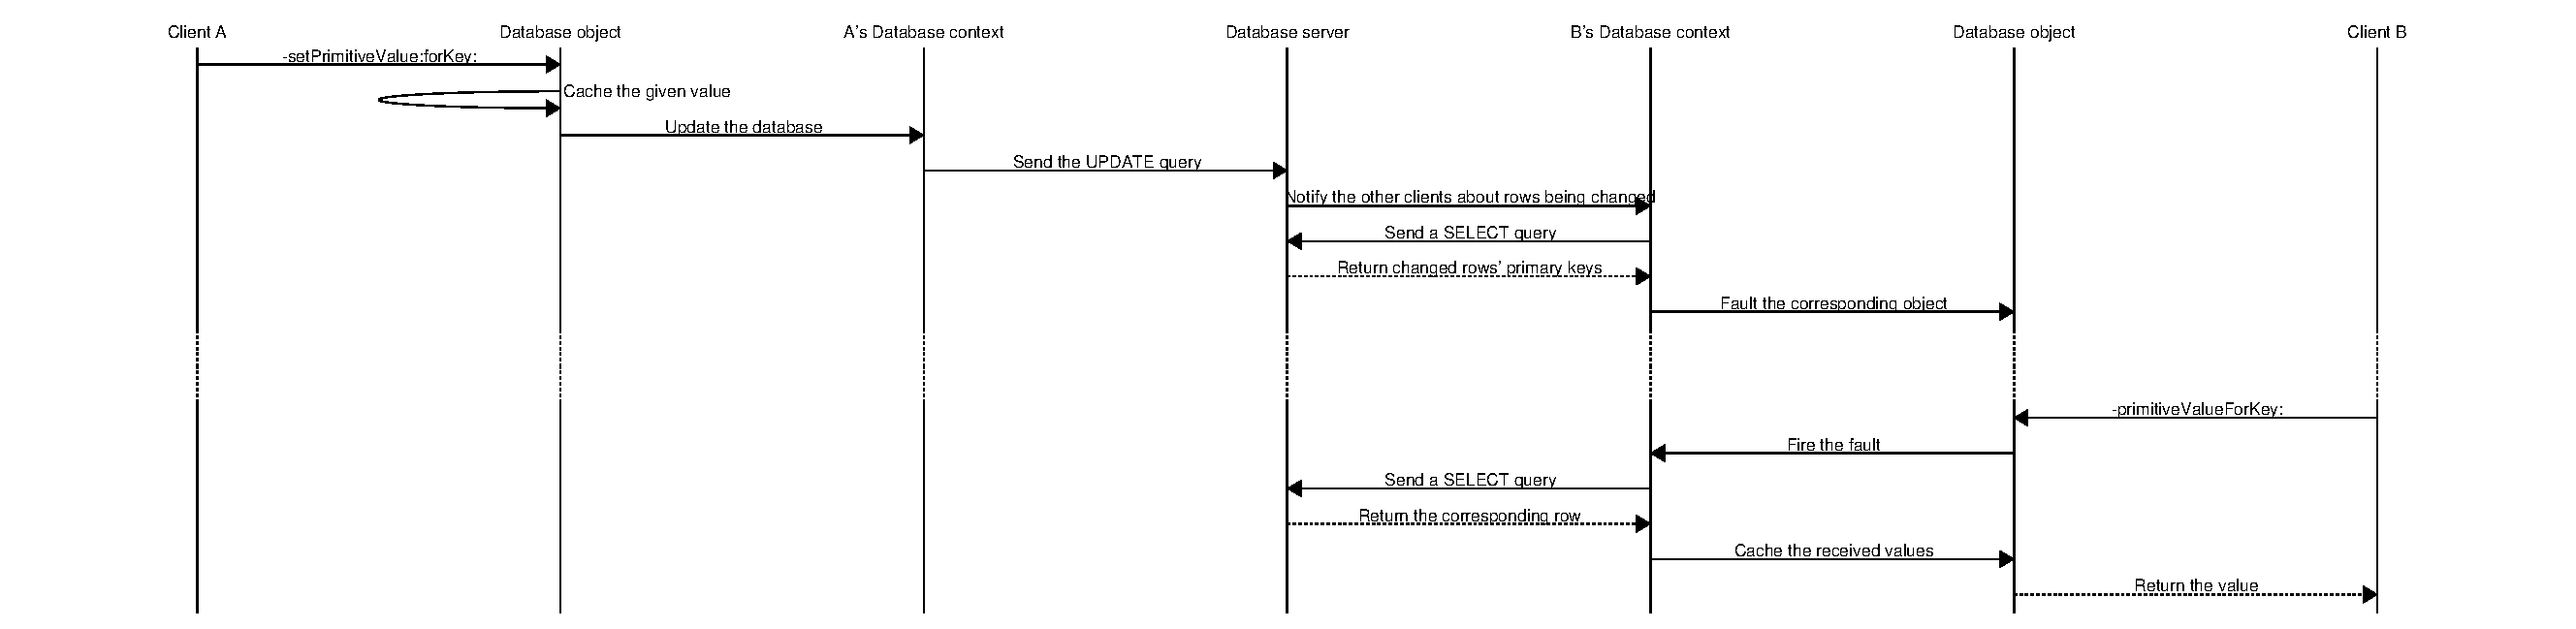
\includegraphics[width=\textheight]{update-change-propagation}
\caption{Objects being accessed by other clients are automatically faulted as part of the update process.}
\end{DoxyImage}
  
\end{sidewaysfigure}
 \hypertarget{sql_views}{}\section{S\+Q\+L views}\label{sql_views}
Contents of S\+Q\+L views may be manipulated using database objects provided that some conditions are met. Unlike tables, views don't have primary keys but Base\+Ten still needs to be able to reference individual rows. If a view has a group of columns that can act as a primary key, the columns may be marked as a primary key with the assistant, after which the view may be enabled.

Views also lack foreign keys. Despite this entities that correspond to views may have relationships provided that a certain condition is met\+: the view needs to have the column or columns of an underlying table that form a foreign key, and the columns' names need to match. In this case, relationships will be created between the view and the target table as well as the view and all the views that are based on the target table and contain the columns the foreign key references to. This applies to the complete view hierarchy.

Postgre\+S\+Q\+L allows I\+N\+S\+E\+R\+T and U\+P\+D\+A\+T\+E queries to target views if rules have been created to handle them. In this case, the view contents may be modified also with Base\+Ten. \hypertarget{database_types}{}\section{Handled Postgre\+S\+Q\+L types}\label{database_types}
Composite types, domains and types not listed here are currently returned as N\+S\+Data. Array types are returned as N\+S\+Arrays of the respective type or N\+S\+Arrays of N\+S\+Data objects.

\begin{table}[h]\begin{TabularC}{2}
\hline
\rowcolor{lightgray}{\bf {\bfseries Postgre\+S\+Q\+L type} }&{\bf {\bfseries Cocoa type}  }\\\cline{1-2}
aclitem &(A private class)  \\\cline{1-2}
bigint, bigserial &N\+S\+Number  \\\cline{1-2}
bit &N\+S\+String  \\\cline{1-2}
boolean &N\+S\+Number  \\\cline{1-2}
bytea &N\+S\+Data  \\\cline{1-2}
char, bpchar &N\+S\+String  \\\cline{1-2}
date &N\+S\+Date  \\\cline{1-2}
decimal, numeric &N\+S\+Decimal\+Number  \\\cline{1-2}
double precision &N\+S\+Number  \\\cline{1-2}
int2vector &N\+S\+Array of N\+S\+Numbers  \\\cline{1-2}
integer, serial &N\+S\+Number  \\\cline{1-2}
name &N\+S\+String  \\\cline{1-2}
oid &N\+S\+Number  \\\cline{1-2}
point &N\+S\+Value  \\\cline{1-2}
real &N\+S\+Number  \\\cline{1-2}
smallint &N\+S\+Number  \\\cline{1-2}
text &N\+S\+String  \\\cline{1-2}
time &N\+S\+Date  \\\cline{1-2}
time with time zone &N\+S\+Date  \\\cline{1-2}
timestamp &N\+S\+Date  \\\cline{1-2}
timestamp with time zone &N\+S\+Date  \\\cline{1-2}
varbit &N\+S\+String  \\\cline{1-2}
varchar &N\+S\+String  \\\cline{1-2}
uuid &N\+S\+String  \\\cline{1-2}
xml &N\+S\+Data or N\+S\+X\+M\+L\+Document  \\\cline{1-2}
\end{TabularNC}
\centering
\caption{Type conversion}
\end{table}
\hypertarget{database_types_string_handling}{}\subsection{String types}\label{database_types_string_handling}
When N\+S\+Strings are passed to the database, they are normalized to Unicode N\+F\+D. In case the database's encoding isn't Unicode (U\+T\+F-\/8), Postgre\+S\+Q\+L will handle the conversion.

Even if the database's encoding is Unicode, Postgre\+S\+Q\+L compares bytes, not Unicode characters, in strings as of version 8.\+3. Thus, comparison within the database could fail when done with non-\/normalized strings or strings in N\+F\+C.\hypertarget{database_types_date_handling}{}\subsection{Date and time types}\label{database_types_date_handling}
Cocoa's and Core Foundation's date classes store the date as seconds from a reference date, 2001-\/01-\/01 00\+:00\+:00 U\+T\+C. S\+Q\+L times and timestamps, on the other hand, might have an associated time zone specified as an offset to G\+M\+T. In Postgre\+S\+Q\+L 8.\+3, removing the time zone information by casting truncates the value. Casting a time or a timestamp lacking a time zone assigns the current time zone to it instead of converting.

Base\+Ten does several things to cope with this\+: \begin{DoxyItemize}
\item It sets the connection's time zone to U\+T\+C. \item It assigns U\+T\+C to times and timestamps that don't have a time zone. \item It converts received times and timestamps in other time zones to U\+T\+C. \item N\+S\+Calendar\+Dates passed as parameters will be converted to U\+T\+C.\end{DoxyItemize}
Therefore, N\+S\+Dates received from the server should in fact contain the offset from their point in time to the reference date. To ease handling, the date is set to 2001-\/01-\/01 in case of time types. This allows -\/\mbox{[}N\+S\+Date time\+Interval\+Since\+Reference\+Date\mbox{]} to return the time's difference to midnight in seconds.

N\+S\+Dates are converted to their date representation using N\+S\+Calendar and its underlying I\+C\+U library. I\+C\+U specifies a single cut-\/over date for the switch from Julian to Gregorian calendar, which is 1582-\/10-\/04. (It isn't currently possible to specify a different cut-\/over date to N\+S\+Calendar.) N\+S\+Dates before this point will be converted to Julian calendar dates. The rationale for this is that timestamps can't be passed directly to Postgre\+S\+Q\+L, and N\+S\+Calendar seems to be the best option for representing timestamps as dates. Postgre\+S\+Q\+L, on the other hand, uses Julian days (number of days since January 1, 4713 B\+C\+E with fraction, length of the year specified as 365.\+2425 days) for date calculations, and most likely converts them to Gregorian calendar dates for presentation. Thus, your mileage may vary when calculating dates within the database.

\begin{DoxyNote}{Note}
In versions earlier than 1.\+7, date handling depended on several factors, such as the current time zone and the server's time zone. This is no longer the case. Also, all date and time types are currently returned as N\+S\+Date, not N\+S\+Calendar\+Date.
\end{DoxyNote}
\hypertarget{database_types_xml_handling}{}\subsection{The X\+M\+L type}\label{database_types_xml_handling}
Postgre\+S\+Q\+L's xml data type handles both X\+M\+L documents and content fragments. Base\+Ten creates N\+S\+Data objects from them by default, but if the table also has a constraint like {\itshape C\+H\+E\+C\+K (xml\+\_\+column I\+S D\+O\+C\+U\+M\+E\+N\+T)}, N\+S\+X\+M\+L\+Documents will be created instead. The constraint mustn't contain any other conditions, but there may be additional C\+H\+E\+C\+K constraints.\hypertarget{database_types_custom_database_types}{}\subsection{Requirements for custom base data types}\label{database_types_custom_database_types}
In case of Base\+Ten-\/enabled tables, column contents are compared on update to determine, which columns did actually change. Thus, any custom base data types (created with {\itshape C\+R\+E\+A\+T\+E T\+Y\+P\+E}) used in these tables need to have the equality operator {\itshape =}. Currently, the operator needs to be accessible using the default search path. In case the custom type is such that the concept of equality doesn't apply, the operator may always return {\itshape false}. In this case the value for the column will always be fetched when the corresponding row changes.

Base\+Ten provides custom equality operators for Postgre\+S\+Q\+L's geometric types, for which the default equality operator would only compare equal areas. \hypertarget{relationships}{}\section{Relationships}\label{relationships}
Base\+Ten supports the same types of relationships as Core Data\+: one-\/to-\/one, one-\/to-\/many and many-\/to-\/many. After Base\+Ten schema has been installed, relationships are created using foreign keys as shown in the following table.

\begin{table}[h]\begin{TabularC}{2}
\hline
\rowcolor{lightgray}{\bf {\bfseries Relationship type} }&{\bf {\bfseries Required conditions}  }\\\cline{1-2}
One-\/to-\/many &A foreign key constraint on the many-\/side.  \\\cline{1-2}
One-\/to-\/one &A foreign key constraint the columns of which also have an unique constraint.  \\\cline{1-2}
Many-\/to-\/many &A helper table that has foreign keys referencing two other tables. The foreign key columns also need to form the table's primary key.  \\\cline{1-2}
\end{TabularNC}
\centering
\caption{Required conditions for relationsips}
\end{table}


\begin{DoxyNote}{Note}
Before Base\+Ten 1.\+8, relationships were only available in enabled tables and views.
\end{DoxyNote}
\hypertarget{relationships_relationship_naming}{}\subsection{Relationship naming}\label{relationships_relationship_naming}
Relationship names are determined from foreign key names. For one-\/to-\/one and one-\/to-\/many relationships, the foreign key's name should have the form {\itshape name1\+\_\+\+\_\+name2}, where {\itshape name1} is the relationship's name from the foreign key's side, and {\itshape name2} is the inverse relationship's name. If the foreign key's name doesn't contain two consecutive underscores, a generated name is used for the inverse relationship. Similarly, if the foreign key's name begins with two underscores, a generated name is used for the relationship. The generated name has the format {\itshape schema\+\_\+table\+\_\+foreignkey}.

Many-\/to-\/many relationships have the same name as the foreign key that references the target table.

Base\+Ten Assistant generates foreign keys with names like this, but if creating or altering the database schema isn't an option, a set of identical relationships is created with different names. Each relationship has the same name as the target table, with the word “\+Set” appended in the case of to-\/many relationships.

The latter naming is also available with views, while the former is not.

In case the two relationships created into the same entity have matching names, the one named after the table and its inverse relationship are removed. In case two relationships created into one entity using different foreign keys have matching names, they will both be removed with their inverse relationships.

\begin{table}[h]\begin{TabularC}{2}
\hline
\rowcolor{lightgray}{\bf {\bfseries Relationship type} }&{\bf {\bfseries Available names}  }\\\cline{1-2}
One-\/to-\/many (inverse, from the foreign key's side) &{\itshape target}Set, first part of the foreign key's name  \\\cline{1-2}
One-\/to-\/many (from the referenced side) &{\itshape target}, second part of the foreign key's name  \\\cline{1-2}
One-\/to-\/one (from the foreign key's side) &{\itshape target}, first part of the foreign key's name  \\\cline{1-2}
One-\/to-\/one (from the referenced side) &{\itshape target}, second part of the foreign key's name  \\\cline{1-2}
Many-\/to-\/many &{\itshape target}Set, name of the foreign key that references the target table  \\\cline{1-2}
\end{TabularNC}
\centering
\caption{Relationship names}
\end{table}


\begin{DoxyNote}{Note}
The relationship names used before version 1.\+7 are still available. They won't be listed by Base\+Ten Assistant, though, and using them will call \hyperlink{_b_x_logger_8h_aebc9da21ce1d8bd8e13dee02d91e1e7d}{B\+X\+Deprecation\+Warning}.
\end{DoxyNote}
\hypertarget{relationships_relationship_naming_example}{}\subsection{Relationship example}\label{relationships_relationship_naming_example}
Consider the following case\+:  
  \lstset{language=SQL, backgroundcolor=\color[rgb]{0.84,0.87,0.90}, rulecolor=\color[gray]{0.53}, frame=single, framesep=0pt, framextopmargin=2pt, framexbottommargin=2pt, fontadjust, columns=fullflexible, captionpos=b}
  \begin{lstlisting}[caption=Tables with a one-to-many relationship]
  CREATE TABLE person (
      id SERIAL PRIMARY KEY,
      firstname VARCHAR (255),
      surname VARCHAR (255)
  );
 
  CREATE TABLE email (
      id SERIAL PRIMARY KEY,
      address VARCHAR (255),
      person_id INTEGER REFERENCES person (id)
  );
  \end{lstlisting} 
   

Lets say we have two objects\+: {\itshape a\+Person} and {\itshape an\+Email} which have been fetched from the person and email tables, respectively.~\newline
 {\ttfamily \mbox{[}a\+Person value\+For\+Key\+:@\char`\"{}email\+Set\char`\"{}\mbox{]}} will now return a collection of {\itshape email} objects.~\newline
 {\ttfamily \mbox{[}an\+Email value\+For\+Key\+:@\char`\"{}person\char`\"{}\mbox{]}} will return a single {\itshape person} object.

If we modify the previous example by adding an unique constraint, we get a one-\/to-\/one relationship\+:

 
  \begin{lstlisting}
  ALTER TABLE email ADD UNIQUE (person_id);
  \end{lstlisting} 
   

Now both of the following messages will return a single object from the corresponding table\+:~\newline
 {\ttfamily \mbox{[}a\+Person value\+For\+Key\+:@\char`\"{}email\char`\"{}\mbox{]}}~\newline
 {\ttfamily \mbox{[}an\+Email value\+For\+Key\+:@\char`\"{}person\char`\"{}\mbox{]}}

Many-\/to-\/many relationships are modeled with helper tables. The helper table needs to have columns to contain both tables' primary keys.

Another example\+:  
  \begin{lstlisting}[caption=Tables with a many-to-many relationship]
  CREATE TABLE person (
      id SERIAL PRIMARY KEY,
      firstname VARCHAR (255),
      surname VARCHAR (255)
  );
 
  CREATE TABLE title (
      id SERIAL PRIMARY KEY,
      name VARCHAR (255)
  );
 
  CREATE TABLE person_title_rel (
      person_id INTEGER REFERENCES person (id),
      title_id INTEGER REFERENCES title (id),
      PRIMARY KEY (person_id, title_id)
  );
  \end{lstlisting} 
   

Lets say {\itshape a\+Person} has been fetched from the person table and {\itshape a\+Title} from the title table. In this case,~\newline
 {\ttfamily \mbox{[}a\+Person value\+For\+Key\+:@\char`\"{}title\+Set\char`\"{}\mbox{]}} will return a collection of title objects and ~\newline
 {\ttfamily \mbox{[}a\+Title value\+For\+Key\+:@\char`\"{}person\+Set\char`\"{}\mbox{]}} a collection of person objects.~\newline
 Any two foreign keys in one table will be interpreted as a many-\/to-\/many relationship, if they also form the table's primary key. Objects from the helper table may be retrieved as with one-\/to-\/many relationships\+:~\newline
 {\ttfamily \mbox{[}a\+Person value\+For\+Key\+:@\char`\"{}person\+\_\+title\+\_\+rel\+Set\char`\"{}\mbox{]}}. \hypertarget{predicates}{}\section{Predicates}\label{predicates}
Cocoa predicates are used to fetch objects that match certain criteria. Key paths in predicates correspond to entity attributes and relationships.

Most types of predicates and expressions are converted to S\+Q\+L and sent to the database server. Others cause the returned object set to be filtered again on the client side. Specifically, the following use cases work in this manner\+: The affected part of the predicate is replaced with {\itshape true} (or {\itshape false}, if the part is inside an odd number of N\+O\+T predicates), and excess objects are removed from the result set after it has been received.


\begin{DoxyItemize}
\item Use of N\+S\+Custom\+Selector\+Predicate\+Operator\+Type 
\item A modifier other than N\+S\+Direct\+Predicate\+Modifier in combination with any of the following\+: 
\begin{DoxyItemize}
\item N\+S\+Begins\+With\+Predicate\+Operator\+Type 
\item N\+S\+Ends\+With\+Predicate\+Operator\+Type 
\item N\+S\+Matches\+Predicate\+Operator\+Type 
\item N\+S\+Like\+Predicate\+Operator\+Type 
\item N\+S\+Contains\+Predicate\+Operator\+Type 
\item N\+S\+In\+Predicate\+Operator\+Type 
\end{DoxyItemize}
\item Use of any of the following predicate options\+: 
\begin{DoxyItemize}
\item N\+S\+Diacritic\+Insensitive\+Predicate\+Option 
\item N\+S\+Normalized\+Predicate\+Option 
\item N\+S\+Locale\+Sensitive\+Predicate\+Option 
\end{DoxyItemize}
\item Use of any of the following expression types\+: 
\begin{DoxyItemize}
\item N\+S\+Subquery\+Expression\+Type 
\item N\+S\+Union\+Set\+Expression\+Type 
\item N\+S\+Intersect\+Set\+Expression\+Type 
\item N\+S\+Minus\+Set\+Expression\+Type 
\item N\+S\+Block\+Expression\+Type 
\end{DoxyItemize}
\item Use of a function expression with a custom target and selector 
\item Use of a function expression with any of the following predefined selectors\+: 
\begin{DoxyItemize}
\item average\+: 
\item cast\+Object\+:to\+Type\+: 
\item max\+: 
\item median\+: 
\item min\+: 
\item mode\+: 
\item random 
\item random\+: 
\item randomn\+: 
\item stddev\+: 
\end{DoxyItemize}
\end{DoxyItemize}\hypertarget{tracking_changes}{}\section{Tracking database changes}\label{tracking_changes}
\hyperlink{interface_b_x_database_object}{B\+X\+Database\+Object} conforms to N\+S\+Key\+Value\+Observing and uses self-\/updating collections for storing related objects; changes in them may thus be tracked with K\+V\+O.

\hyperlink{interface_b_x_synchronized_array_controller}{B\+X\+Synchronized\+Array\+Controller}'s contents will be updated automatically. B\+X\+Database\+Context's fetch methods also have the option to return a self-\/updating array instead of an ordinary one. In this case, the collection's owner has to be specified for K\+V\+O notifications to be posted. See the collection classes' documentation for details.

Another, a more low-\/level means of tracking changes is observing N\+S\+Notifications. Notifications on entity changes will be posted to the relevant context's notification center. The notification object will be a \hyperlink{interface_b_x_entity_description}{B\+X\+Entity\+Description} which corresponds to the table where the change happened. The names of the notifications are\+: \begin{DoxyItemize}
\item {\itshape k\+B\+X\+Insert\+Notification} on database {\itshape I\+N\+S\+E\+R\+T} \item {\itshape k\+B\+X\+Update\+Notification} on database {\itshape U\+P\+D\+A\+T\+E} \item {\itshape k\+B\+X\+Delete\+Notification} on database {\itshape D\+E\+L\+E\+T\+E}\end{DoxyItemize}
At the time the notifications are posted, database objects and self-\/updating collections will already have been updated.\hypertarget{tracking_changes_trigger_effects}{}\subsection{Effects of triggers}\label{tracking_changes_trigger_effects}
When inserting, updating or deleting rows, Base\+Ten notices (and posts notifications of) changes that occur as a result of database triggers or rules firing. The only requirement is that said changes are to entities other than the one being changed by Base\+Ten; changes to the same entity will be ignored. \hypertarget{using_appkit_classes}{}\section{Using Base\+Ten\+App\+Kit}\label{using_appkit_classes}
When Base\+Ten\+App\+Kit is linked to an application, B\+X\+Database\+Context gains some additional capabilities. If given a partial database U\+R\+I, it will present a number of connection panels when -\/connect\+: is called.

B\+X\+Database\+Objects may be used much in the same manner as N\+S\+Managed\+Objects to populate various Cocoa views. To handle some situations unique to Base\+Ten, some N\+S\+Controller subclasses have been provided with the framework. For now, the only directly usable one is \hyperlink{interface_b_x_synchronized_array_controller}{B\+X\+Synchronized\+Array\+Controller}. Additionally, there is \hyperlink{protocol_b_x_controller-p}{B\+X\+Controller} and additions to N\+S\+Controller for creating controller subclasses.

Base\+Ten\+App\+Kit contains a plug-\/in for Interface Builder. The plug-\/in should get loaded automatically if the framework is added to a project.

\begin{DoxyNote}{Note}
Under some circumstances the outlets and actions won't show up when the plug-\/in has been loaded for the first time. If this happens, save and close your document and open it again. Also relaunching Interface Builder has solved the issue.
\end{DoxyNote}
\hypertarget{using_appkit_classes_bxsynchronizedarraycontroller}{}\subsection{B\+X\+Synchronized\+Array\+Controller}\label{using_appkit_classes_bxsynchronizedarraycontroller}
Compared to N\+S\+Array\+Controller, \hyperlink{interface_b_x_synchronized_array_controller}{B\+X\+Synchronized\+Array\+Controller} can do the following things\+: 
\begin{DoxyItemize}
\item It can present errors to the user when creating a new object fails. 
\item It can get a \hyperlink{interface_b_x_entity_description}{B\+X\+Entity\+Description} from its database context and fetch objects using it. N\+S\+Entity\+Descriptions cannot be used because they are Core\+Data-\/specific. 
\item It can lock the edited row in the database when an editing session begins. 
\item It can provide the selected objects' ids. 
\end{DoxyItemize}

\hyperlink{interface_b_x_synchronized_array_controller}{B\+X\+Synchronized\+Array\+Controller} shouldn't be set to entity mode; the user interface for this isn't even available in Interface Builder. It also doesn't make use of a managed object context.

\hyperlink{interface_b_x_synchronized_array_controller}{B\+X\+Synchronized\+Array\+Controller}'s Content Set may be bound to another synchronized array controller with a key path that represents a relationship. In case of a one-\/to-\/many relationship, the foreign key field values will also be set when -\/new\+Object or -\/create\+Object\+: gets called.\hypertarget{using_appkit_classes_using_bxdatabasecontext_ib}{}\subsection{Using B\+X\+Database\+Context from Interface Builder}\label{using_appkit_classes_using_bxdatabasecontext_ib}

\begin{DoxyEnumerate}
\item Load the Base\+Ten plug-\/in. 
\item Create a new nib file. 
\item Drag a database context from the library to the file. 
\item Select the database context and choose Attributes from the inspector's pop-\/up menu. 
\item Enter a valid database U\+R\+I, {\ttfamily pgsql\+:///{\itshape database\+\_\+name}} at minimum. 
\end{DoxyEnumerate}\hypertarget{using_appkit_classes_using_bxsynchronizedarraycontroller_ib}{}\subsection{Using B\+X\+Synchronized\+Array\+Controller from Interface Builder}\label{using_appkit_classes_using_bxsynchronizedarraycontroller_ib}

\begin{DoxyEnumerate}
\item Drag a \hyperlink{interface_b_x_synchronized_array_controller}{B\+X\+Synchronized\+Array\+Controller} from the library to the file. 
\item Select the array controller and choose Attributes from the inspector's pop-\/up menu. 
\item Enter a table name into the field. 
\begin{DoxyItemize}
\item The schema field may be left empty, in which case {\itshape public} will be used. 
\end{DoxyItemize}
\item Bind the Cocoa views to the controller. 
\item Bind the array controller to the database context using the Database Context binding or connect the database\+Context outlet. 
\item Test the interface. The views should be populated using the database. 
\end{DoxyEnumerate}\hypertarget{using_appkit_classes_using_value_transformers_ib}{}\subsection{Using Base\+Ten\+App\+Kit's value transformers from Interface Builder}\label{using_appkit_classes_using_value_transformers_ib}
When database rows get locked, it might be desirable to disable editing and indicate this visually in the user interface. Most App\+Kit's classes, have an Editable binding, and some, like N\+S\+Table\+Column, have bindings that affect the display of their value. Lets say a table column's {\itshape Value} is bound to a B\+X\+Array\+Controller using {\itshape my\+\_\+key} as the model key path. Base\+Ten\+App\+Kit could then be used to set the rows to be conditionally editable like this\+: 
\begin{DoxyEnumerate}
\item Select the table column inside its table view 
\item Open the Bindings Inspector 
\item Click the Editable binding 
\item Set the binding to the array controller and set the controller key to {\itshape arranged\+Objects}. 
\item Set the model key to {\itshape status\+Info.\+my\+\_\+key}. 
\item Set the value transformer to {\itshape \hyperlink{interface_b_x_object_status_to_editable_transformer}{B\+X\+Object\+Status\+To\+Editable\+Transformer}}. 
\end{DoxyEnumerate}The rows may also be coloured so that their status is visible\+: 
\begin{DoxyEnumerate}
\item Inspecting the same column as in the previous example, click the Text Color binding. 
\item Set the binding to the array controller and set the controller key to {\itshape arranged\+Objects}. 
\item Set the model key to {\itshape status\+Info.\+my\+\_\+key}. 
\item Set the value transformer to {\itshape \hyperlink{interface_b_x_object_status_to_color_transformer}{B\+X\+Object\+Status\+To\+Color\+Transformer}}. 
\end{DoxyEnumerate}\hypertarget{autocommit_manual_commit}{}\section{Commit modes and locking}\label{autocommit_manual_commit}
B\+X\+Database\+Context has two modes for handling transactions, which affect queries sent to the database and the way the context's undo manager is used. In both cases, the transaction isolation level is set to R\+E\+A\+D C\+O\+M\+M\+I\+T\+T\+E\+D meaning that changes committed by other connections will be received. The commit mode is set using -\/set\+Autocommits\+:. Generally, autocommit is well-\/suited for non-\/document-\/based applications. Manual commit is well-\/suited for document-\/based applications, provided that changes are committed frequently enough.\hypertarget{autocommit_manual_commit_autocommit}{}\subsection{Autocommit}\label{autocommit_manual_commit_autocommit}
When using autocommit, each query creates its own transaction and changes get propagated immediately to other clients. Undo works at the level of -\/\mbox{[}\hyperlink{interface_b_x_database_object}{B\+X\+Database\+Object} set\+Primitive\+Value\+:for\+Key\+:\mbox{]}. For each change an invocation of the method is added to the undo manager with the earlier value as a parameter.\hypertarget{autocommit_manual_commit_manual_commit}{}\subsection{Manual commit}\label{autocommit_manual_commit_manual_commit}
In manual commit mode, a savepoint is added after each change. Undo causes a R\+O\+L\+L\+B\+A\+C\+K T\+O S\+A\+V\+E\+P\+O\+I\+N\+T query to be sent. This causes not only the changes made by Base\+Ten to be reverted, but their possible side effects as well. For instance, if database triggers fire when a specific change is made, its effects will be reverted, too. When -\/commit\+: or -\/rollback is called, undo queue is emptied.

In case one client updates a row, Base\+Ten doesn't send the change to other clients immediately. Instead, it sends a notification indicating that the row is locked and changing it will cause the connection to block until the other client ends its transaction. \hyperlink{interface_b_x_database_object}{B\+X\+Database\+Object}'s method -\/is\+Locked\+For\+Key\+:, B\+X\+Database\+Object\+Status\+Info class and value transformers in Base\+Ten\+App\+Kit are useful for handling this situation. However, other than Base\+Ten clients don't cause the lock status to be set, and the connection could block.

The downside is that if -\/\mbox{[}B\+X\+Database\+Context commit\+:\mbox{]} or -\/\mbox{[}B\+X\+Database\+Context rollback\mbox{]} aren't called frequently enough, transactions could become very long, which is against their intended use. This causes server resources to be consumed.\hypertarget{autocommit_manual_commit_locking_rows}{}\subsection{Locking rows}\label{autocommit_manual_commit_locking_rows}
When a database connection sends U\+P\+D\+A\+T\+E and D\+E\+L\+E\+T\+E queries, the affected rows will be locked until the connection ends its transaction. If other connections try to change the rows, their queries will block. To handle this situation, Base\+Ten stores information about locked rows into its internal tables and notifies other Base\+Ten clients about them. \hyperlink{interface_b_x_synchronized_array_controller}{B\+X\+Synchronized\+Array\+Controller} also tries to lock rows when the editing session begins.

Lock information will be available using \hyperlink{interface_b_x_database_object}{B\+X\+Database\+Object}'s method -\/is\+Locked\+For\+Key\+:. B\+X\+Database\+Context has a method, -\/set\+Sends\+Lock\+Queries\+:, for enabling or disabling lock notifications. If the notifications are disabled, B\+X\+Database\+Context won't notify other clients but still reacts to received notifications.

When editing rows through \hyperlink{interface_b_x_synchronized_array_controller}{B\+X\+Synchronized\+Array\+Controller}, it tries to send a S\+E\+L\+E\+C\+T ... F\+O\+R U\+P\+D\+A\+T\+E N\+O\+W\+A\+I\+T query when the editing session begins. If the context is in autocommit mode, a transaction will also be started. If the query succeeds, a lock notification will be sent regardless of B\+X\+Database\+Context's setting. If the query fails, the editing session will be ended using -\/discard\+Editing. \hyperlink{interface_b_x_synchronized_array_controller}{B\+X\+Synchronized\+Array\+Controller}'s method -\/set\+Locks\+Rows\+On\+Begin\+Editing\+: can be used to disable this functionality.

To make the changes visible in the user interface, Base\+Ten\+App\+Kit has some N\+S\+Value\+Transformer subclasses. See \hyperlink{group__value__transformers}{Value Transformers} for details. \hypertarget{thread_safety}{}\section{Thread safety}\label{thread_safety}
For its mostly used parts, Base\+Ten isn't thread safe. In particular, B\+X\+Database\+Context needs to be used from the same thread in which its connection methods have been called. This is because it adds a run loop source to the thread's run loop.

The documented methods of the following classes are thread safe\+:

\begin{DoxyItemize}
\item \hyperlink{interface_b_x_entity_description}{B\+X\+Entity\+Description} \item \hyperlink{interface_b_x_attribute_description}{B\+X\+Attribute\+Description} \item \hyperlink{interface_b_x_relationship_description}{B\+X\+Relationship\+Description} \item \hyperlink{interface_b_x_database_object_i_d}{B\+X\+Database\+Object\+I\+D}\end{DoxyItemize}
Additionally, \hyperlink{interface_b_x_database_object}{B\+X\+Database\+Object}'s method -\/cached\+Value\+For\+Key\+: is thread safe. As a result, \hyperlink{interface_b_x_database_object}{B\+X\+Database\+Object}'s values may be accessed from multiple threads as soon as they have been fetched.

One possibility to make use of multiple threads is to create a database context for each thread, but see \hyperlink{multiple_contexts}{the next chapter}. \hypertarget{multiple_contexts}{}\section{Using multiple database contexts}\label{multiple_contexts}
In general, there aren't many reasons to have multiple database contexts in an application that connects to a single database. One possibility to make the context available everywhere it's needed is to make it a property of the N\+S\+Application delegate or an N\+S\+Document subclass.

Advantages\+: \begin{DoxyItemize}
\item Thread safety. Since database contexts should be created and used from within a single thread, it might be advantageous to create one for each thread. \item Transaction isolation. One could want to query the database state outside the current transaction. \item Privilege separation. One might want to access the database using roles with different privileges. \item Different commit modes.\end{DoxyItemize}
Disadvantages\+: \begin{DoxyItemize}
\item Increased memory usage on the server. Each database context makes a connection to the database (two in manual commit mode). These require an amount of shared memory on the server. This limits the number of clients who can connect simultaneously. \item Increased memory and network usage on the client side. Database objects are uniqued and updated within a context, so each context requires its own copy of the objects. Each context also needs to update its objects on its own. \item Database objects cannot be passed from one context to another. This causes problems. \end{DoxyItemize}
\hypertarget{linking_to_baseten}{}\section{Linking to Base\+Ten and Base\+Ten\+App\+Kit}\label{linking_to_baseten}
Mac O\+S X's linker specifies paths to dynamic libraries (including frameworks) using a the install name of the library. The install name is specified in the library itself. Base\+Ten and Base\+Ten\+App\+Kit distributed on the disk image have their install names set to a location inside the loading application's bundle, in the Frameworks folder. When linking to the frameworks in Xcode, a Copy Files build phase should be added for the application target\+: 
\begin{DoxyEnumerate}
\item Right-\/click your application target in the Groups \& Files table 
\item Select Add, New Build Phase and New Copy Files Build Phase 
\item Select Frameworks as the destination 
\item Click the disclosure triangle next to your target 
\item Drag Base\+Ten and Base\+Ten\+App\+Kit inside the new build phase 
\end{DoxyEnumerate}

The frameworks are built with the -\/headerpad\+\_\+max\+\_\+install\+\_\+names linker option, so changing the install names with tools like install\+\_\+name\+\_\+tool should also be possible. When building Base\+Ten and Base\+Ten\+App\+Kit using the Debug configuration, the install name is left empty, which causes it to be set to the build directory. \hypertarget{building_baseten}{}\section{Building Base\+Ten}\label{building_baseten}
For a successful build, Xcode 3.\+1 and Mac O\+S X 10.\+5 S\+D\+K are required.

Base\+Ten has several subprojects, namely Base\+Ten\+App\+Kit and a plug-\/in for Interface Builder 3. The default target in Base\+Ten.\+xcodeproj, {\itshape Base\+Ten + G\+C}, builds them as well; the plug-\/in and the App\+Kit framework will appear in the subprojects' build folders, which are set to the default folder. The built files will be either in {\itshape build} folders in the subprojects' folders or in the user-\/specified build folder. The documentation will be in the {\itshape Documentation} folder.\hypertarget{building_baseten_building_for_the_release_dmg}{}\subsection{Building for the release disk image}\label{building_baseten_building_for_the_release_dmg}
The files needed to build the release disk image are in the S\+V\+N repository as well. Doxygen is needed during the process. To create the D\+M\+G, follow these steps\+: 
\begin{DoxyEnumerate}
\item From the checked-\/out directory, {\ttfamily cd Release\+D\+M\+G}. 
\item The default location for the built files is {\itshape Base\+Ten-\/dmg-\/build} in the current directory. To set a custom path, edit the {\itshape S\+Y\+M\+R\+O\+O\+T} variable in {\itshape create\+\_\+release\+\_\+dmg.\+sh}. 
\item Do {\ttfamily ./create\+\_\+release\+\_\+dmg.sh}. The built D\+M\+G will appear in the {\itshape Release\+D\+M\+G} folder. 
\begin{DoxyItemize}
\item If you don't have La\+Te\+X installed, do {\ttfamily ./create\+\_\+release\+\_\+dmg.sh -\/--without-\/latex} instead. The P\+D\+F manual won't be included on the D\+M\+G, though. 
\end{DoxyItemize}
\end{DoxyEnumerate}